\documentclass{article}
\usepackage{graphicx}
\begin{document}
{\large {\bfseries Genomic sequence alignment with motif anchors.}}
\begin{abstract}
{\large Motivation:} Comparative sequence analysis is the essence of many approaches to genome annotation. Heuristic alignment algorithms utilize similar seed pairs to anchor an alignment. Some applications of local alignment algorithms (e.g. phylogenetic footprinting) would benefit from including prior knowledge (e.g. binding site motifs) in the alignment building process.
\\
{\large Results:} We introduce predefined sequence patterns as anchor points into a heuristic local alignment strategy. We extended the BLASTZ program for this purpose. A set of seed patterns is either given as consensus sequences in IUPAC code or position-weight-matrices (PWMs). Phylogenetic footprinting of promoter regions is one of many potential application for the SITEBLAST software.
\end{abstract}
\subsection*{SITEBLAST commandline options}
We will only discuss command line options that differ from the original BLASTZ distribution as in {\tt http://www.bx.psu.edu/miller\_lab/}.
\\
Usually, the program is invoked by typing
\begin{verbatim}
siteblast seq1 [seq2] options
\end{verbatim}
where options can be one of the following and/or the standard {\tt BLASTZ} options. Sequence data must be given in capital letters.
\subsubsection*{Switch A, Printing option}
This switch takes values from 1 - 3. To get a BLASTZ-like condensed output format choose 1.\\
In case you look for some well-formated output, try the pretty print option and choose 2.\\
\begin{verbatim}
378  .    :    .    :    .    :     .    :    .    :    .
GCGAGCAGTTCCCGTCAATCCCTCCCCCCTT-ACACAGGATGTCCATATTAGGACATCTG
GCGAGCTGTTCCCGTCAATCCCTCCCTCCTTTACACAGGATGTCCATATTAGGACATCTG
201  .    :    .    :    .    :    .    :    .    :    .
  ^^^^^^^^^^P53 (sense) dist:2|2
  ^^^^^^^^^^P53 (rev. cmpl) dist:2|2
         ^^^^^^^^CREB (sense) dist:2|2
         ^^^^^^^^CREB (rev. cmpl) dist:2|2
           ^^^^^^^^E2F (rev. cmpl) dist:2|2
           ^^^^^^^^ELK1 (sense) dist:2|2
              ELK1 (sense) dist:2|2^^^^^^^^
               P53 (sense) dist:2|2^^^^^^^^^^
           P53 (rev. cmpl) dist:2|2^^^^^^^^^^
                       SRF (sense) dist:1|1^^^^^^^^^^
                   SRF (rev. cmpl) dist:1|1^^^^^^^^^^
                       CREB (rev. cmpl) dist:2|2^^^^^^^^
                               P53 (sense) dist:2|2^^^^^^^^^
                           P53 (rev. cmpl) dist:2|2^^^^^^^^^
                                CREB (rev. cmpl) dist:2|2^^^
                                  AP1 (rev. cmpl) dist:2|2^^

437  .    :    .    :    .    :    .    :      .    :    .
CGTCAGCAGGTTTCCACGGCCTTTCCCTGTAGCCCTGGGGGGAG--CCATCCCCGAAACC
CGTCAGCAGGTTTCCACGGCCGGTCCCTGTTGTTCTGGGGGGGGGACCATCTCCGAAATC
261  .    :    .    :    .    :    .    :    .    :    .
^P53 (sense) dist:2|2
^P53 (rev. cmpl) dist:2|2
^^^^^CREB (rev. cmpl) dist:2|2
^^^^^^^AP1 (rev. cmpl) dist:2|2
   ^^^^^^^^^^P53 (sense) dist:2|2
   ^^^^^^^^^^P53 (rev. cmpl) dist:2|2
\end{verbatim}
Choose 3 for both. The pretty-print option generates pairwise alignment output, which is decorated with all found anchor points.
\subsubsection*{Switch I, IUPAC seeds - key word tree search}
This option takes a filename as argument. The file should contain two tab-seperated columns:
\begin{verbatim}
TGACGTMA        CREB
CCAWATAWGG      SRF
....
\end{verbatim}
First column holds a consensus motif expressed in IUPAC symbols. Second column holds a unique identifier to this motif.
\begin{verbatim}
Example: siteblast seq1 seq2 I=somedirectory/somefile
\end{verbatim}
Kindly note that seed pairs do not need to be identical.
For example, valid seed pairs for consensus pattern {\tt CCWWWWWWGG} include CCATAATAGG - CCATTTTAGG.
\subsubsection*{Switch i, IUPAC seeds - trivial search}
Same as switch I. However, the search strategy differs. A trivial search is run over the entire input sequences to find seeds.
\subsubsection*{Switch D, Distance to IUPAC seeds.}
This option sets the number of allowed mismatches of an individual seed point to the given consensus description as given by the i option or the I option. In other words, subsequences that deviate from the consensus in $D$ positions are still considered as seeds. These seeds will be subsequently employed in alignment building.\\
Allowing for additional mismatches leads to the acceptance of more subsequences as seed pairs. For example,  valid seed pairs for consensus pattern {\tt CCWWWWWWGG} include CCATAATAGG - CCATTTTAGG for $D=0$ and ACATAATAGG - CCATTTTAGG for $D=1$.
\subsubsection*{Switch P, Seed search with position-weight-matrices}
If set, this option reads in a set of position-weight-matrices (PWMs, all in one file). The format of a matrix entry is shown below:
\begin{verbatim}
>E2F-1|E2F-1  8
0.076721890299285 0.22663524926424 0.155128754560068 0.541514105876407
0.00183623473089011 0.0774357961198575 0.187190918506619 0.733537050642633
0.111301251090967 0.00168889040931061 0.00168889040931061 0.885320968090412
0.00250289974347753 0.588549446853129 0.406444753659916 0.00250289974347753
0.00238495824006619 0.333590174989956 0.661639908529912 0.00238495824006619
0.001729434010637 0.882689533127682 0.113851598851044 0.001729434010637
0.001729434010637 0.113851598851044 0.882689533127682 0.001729434010637
0.00414116507322938 0.621920691570233 0.333779304956604 0.040158838399933
<
\end{verbatim}
Both sequences are scanned for matches to the set of matrices with individual background models (due to different GC-content). The algorithm tries to combine hits(seeds) from the same matrix in both sequences into anchor points. Then, alignments are built from the anchor point collection.

\subsubsection*{Switch pValue(required) and powerLimit(optional)}
To identify seeds by PWM scans, one has to discriminate true from false positives. The pValue option sets the proportion of accepted false positives (blue area in image below). This pValue is divided by the length of the scanned sequence to adjust for multiple testing. A limit on the power (proportion of true positives) can be set optionally. In short, one fixes a $p-value$ for all matrices and is free to add a lower boundary on the power (area under signal curve above score threshold).\\
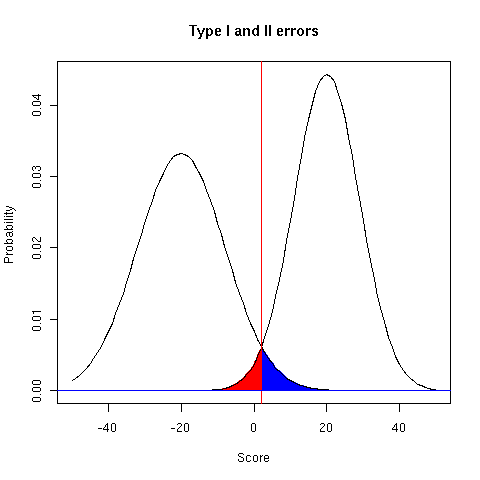
\includegraphics{typeIandII}
\begin{verbatim}
Commandline options are:
-pValue=]0,0.1[
-powerLimit
\end{verbatim}
\subsubsection*{Switch power(required) and pValueLimit(optional)}
Alternatively, one can fix a lower power bound and add an upper bound on the $p-value$.
\begin{verbatim}
Commandline options are:
-power=]0,1[
-pValueLimit
\end{verbatim}

\subsection*{Copyright and license agreement}
Permission to use any part of our software for educational, research and non-profit purposes, without fee, and without a written agreement is hereby granted, provided that the copyright notice (Copyright (c) 2001-2004 Max Planck Society, All Rights Reserved), this paragraph and the following two paragraphs appear in all copies.

IN NO EVENT SHALL THE MAX PLANCK SOCIETY BE LIABLE TO ANY PARTY
FOR DIRECT, INDIRECT, SPECIAL, INCIDENTAL, OR CONSEQUENTIAL DAMAGES,
INCLUDING LOST PROFITS, ARISING OUT OF THE USE OF OUR SOFTWARE,
EVEN IF THE MAX PLANCK SOCIETY HAS BEEN ADVISED OF THE
POSSIBILITY OF SUCH DAMAGE.

THE SOFTWARE PROVIDED HEREIN IS ON AN "AS IS" BASIS, AND
THE MAX PLANCK SOCIETY HAS NO OBLIGATION TO PROVIDE MAINTENANCE,
SUPPORT, UPDATES, ENHANCEMENTS, OR MODIFICATIONS.  THE MAX PLANCK SOCIETY
MAKES NO REPRESENTATIONS AND EXTENDS NO WARRANTIES OF ANY
KIND, EITHER IMPLIED OR EXPRESSED, INCLUDING, BUT NOT LIMITED TO, THE
IMPLIED WARRANTIES OF MERCHANTABILITY OR FITNESS FOR A PARTICULAR
PURPOSE, OR THAT THE USE OF OUR SOFTWARE WILL NOT INFRINGE
ANY PATENT, TRADEMARK OR OTHER RIGHTS.

\end{document}


